\documentclass[10pt]{article}

\usepackage[utf8]{inputenc}
\usepackage{floatrow}

\usepackage{algorithm}
\usepackage{algorithmic}
\usepackage[T1]{fontenc}
\usepackage{enumitem}
\usepackage{hyperref}
\usepackage{graphicx}
\usepackage{color}
\usepackage{listings}
\usepackage{wrapfig}
\usepackage[hmargin=1.25in,vmargin=1.25in]{geometry}

%title setup
\title{Projet IPI: chemins de poids minimum}
\author{Romain PEREIRA}
\date{04/12/2017}

% table of contents setup
\renewcommand{\contentsname}{Sommaire}
\usepackage{etoolbox}
\patchcmd{\thebibliography}{\section*{\refname}}{}{}{}

\hypersetup{
    colorlinks,
    citecolor=black,
    filecolor=black,
    linkcolor=blue,
    urlcolor=red
}
			
\begin{document}
	\maketitle
	\tableofcontents

	\section*{Préambule}

		Ce projet est réalisé dans le cadre de mes études à l'ENSIIE.\newline Le but est d'implémenter des
		algorithmes de recherche de 'chemin le plus court', dans des graphes orientés.
		Ce document rapporte mon travail, et explique les choix techniques qui ont été pris.
		Soit (X, A) un graphe. On note:
		\begin{itemize}[label=-]
			\setlength\itemsep{0.1em}
			\item X : sommets du graphe
			\item A : arcs du graphe
			\item n : Card(X)
			\item s : sommet 'source', celui à partir duquelle les chemins sont construits
			\item t : sommet 'target', celui vers lequel on souhaite construire un chemin
		\end{itemize}

		\begin{figure}
			\floatbox[{\capbeside\thisfloatsetup{capbesideposition={right,top},capbesidewidth=6cm}}]{figure}[\FBwidth]
			{\caption{\textit{\newline graphe G n=7, \newline X=\{1, 2, ... 7\}, \newline A=\{(1, 4), (4, 6), ... (6, 7)\}}}
			\label{fig:test}}
			{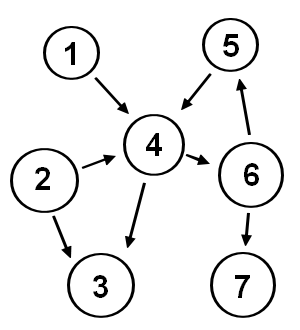
\includegraphics[height=2cm]{./images/graph.png}}
		\end{figure}

	\newpage
	\section{Recherche de chemin le plus court}
		\subsection{Parcours en largeur (graphes non-pondérés)}
			On considère ici un graphe où les arcs sont non pondérés. 'Le chemin le plus court'
			entre 2 sommets corresponds à une famille d'arcs, dont le cardinal est minimum.
			On souhaite codder l'information:
			\begin{itemize}[label=-]
				\item `il existe un arc entre le sommet 'u' et le sommet 'v' `
			\end{itemize}
			Cette information est un booléen, et peut donc être coddée sur un bit.
			J'économise ainsi beaucoup de mémoire. (8 fois plus que si l'arc était coddé sur un octet),
			en representant mes arcs sur un tableau de bit. Soit 'b' l'indice d'un bit dans un tableau d'octet.
			Pour y accéder, il faut récuperer l'indice $\textrm{b}_\textrm{o}$ de l'octet correspondant dans le tableau,
			et l'indice $\textrm{b}_\textrm{b}$ du bit sur cet octet.\newline
			En posant:
			\begin{itemize}[label=-]
				\item \(b_o = b / 8\) (quotient de la division euclidienne de 'b' par 8
				\item \(b_b = b \% 8\) (reste de la division euclidienne de 'b' par 8
			\end{itemize}
			on s'assure de l'unicité,
			\begin{itemize}[label=-]
				\item \(b = 8*b_o+b_b\)
			\end{itemize}
			On peut aussi faire une transformation entre 2 sommets ('u', 'v') vers un bit 'b'.

			\begin{itemize}[label=-]
				\item \(u = b \% n\)
				\item \(v = b / n\)
				\item \(b = n * v + u\)
			\end{itemize}
			
			Le bit 'b' vaux 1 s'il existe un arc entre 'u' et 'v', 0 sinon.
			On a besoin de \(n^2\) bits, et donc de \(n^2 / 8 + 1\) octets.
			On gagne donc 8 fois plus de mémoire que si l'information était stocké sur un octet.
			De plus, je ne perd pas de temps en lecture / écriture dans le tableau des arcs, car ces changements
			de coordonnées ne necessite que 1 multiplication, 1 addition, et quelques operations sur les bits (diviser par 8 <=> décaler
			les bits de 3 vers la droite)
			
			Egalement, en réduisant la mémoire utilisé, je rends mon programme plus `cache-friendly`, le rendant plus rapide.
			Le processeur écrit des blocs mémoire du programme dans sa mémoire cache: plus les données sont compactes,
			moins il aura à faire des allés/retours entre la mémoire du programme et sa mémoire cache.\newline
							
			\begin{wrapfigure}{R}{5cm}
				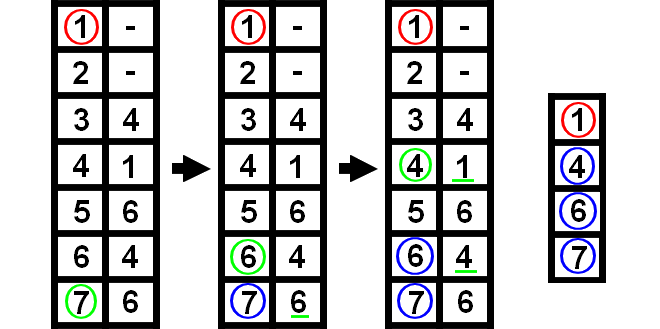
\includegraphics[width=5cm]{./images/remonte.png}
				\caption{\textit{Schéma de l'algorithme de remonté}}
			\end{wrapfigure}

			Chaque sommet 'u' de mon graphe possède un attribut pointant vers un autre sommet du graphe.
			Une fois l'algorithme de parcours terminé, cet attribut pointe vers le prédécesseur de 'u',
			dans le chemin le plus court allant de 's' à 't', et passant par 'u'.
			Pour reconstruire le chemin, il suffit de regarder recursivement les prédécesseurs, en partant du sommet
			't' jusqu'à ce que l'on ait atteint 's'.
			La complexité de la reconstruction est en O(m), où 'm' est la longueur du chemin.\newline
			
			Cette modélisation permet de réduire les coûts de stockage, et la remonté est d'un coût
			négligeable devant le temps de résolution du chemin. Elle sera réutiliser dans Dijkstra et A*.
			
		\subsection{Algorithme de Dijkstra (graphes pondérés positivement)}
			On considère ici un graphe où les arcs sont pondérés avec des poids positifs.\newline
			'Le chemin le plus court' entre 2 sommets corresponds au chemin avec la somme des poids de ses arcs minimum.\newline
			L'algorithme de Dijkstra nous est fourni dans le sujet. Remarquons que si le poids de tous les arcs sont identiques,
			on retrouve l'algorithme de parcours en largeur.
			\subsubsection{1ère approche}
				Ma 1ère implementation reprends le squelette du parcours en largeur.\newline\newline
				On remplace le tableau de bit par une matrice d'entier (4 octets), stockant le poids des arcs.\newline\newline
				Cependant, une différence réside dans le choix du prochain sommet à visiter. Dans le parcours en largeur,
				les sommets sont visités dans leur ordre d'apparation dans la liste (1er entré, 1er sorti).
				Trouver le prochain sommet à visiter est d'une complexité \textbf{\(O(1)\)}.
				Dans l'algorithme de Dijkstra, les sommets sont visités par ordre du poids de leur chemin à 's'.
				Ainsi, si la file de visite contient 'm' sommets, trouver le prochain sommet
				à visiter devient en complexité \(O(m)\)

			\subsubsection{2ème approche}								
				En utilisant une matrice, la complexité ('spatial') de stockage des arcs est donc en \(O(n^2)\).
				Plus précisement, si le poids est stocké sur 4 octet, pour \(n=10^6\) (cas labyrinthe exo3/tests/06),
				l'espace mémoire nécessaire est de \(400Go\)... On va donc changer de structures de données.
				En ajoutant un attribut liste à chaque sommet, qui contient l'indice de ses sommets voisins,
				la complexité spatial devient devient donc (au plus) en \(m * O(n)\), où 'm' est
				le nombre maximal de successeurs par sommet. (Remarque : pour \(m = n\), on retrouve \(O(n^2)\))
				Il en résulte que dans la résolution de labyrinthe (exo3/tests/06), on a \(m <= 5\), donc pour \(n=10^6\),
				on passe donc de \(400Go\) à \(5 Mo\).
				
			\subsubsection{File de priorité ('Priority Queue')}
			
				Après avoir implementé Dijkstra avec cette 2nde approche, j'ai étudié le temps d'execution.
				\begin{figure}[H]
					\begin{center}
						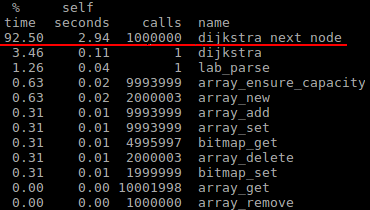
\includegraphics[width=6cm,height=\textheight,keepaspectratio]{./images/no_pqueue.png}
					\end{center}
				    \caption{\textit{résultat de 'gprof' sur 'tests/exo3/06'}}
				\end{figure}
				Il s'est avéré que mon programme passe (en moyenne) plus de 70\% de
				son temps d'execution à chercher le prochain sommet à visiter.
				(l'opération `trouver un sommet 'u' non visité minimisant 'd(u)` dans l'algorithme fourni).\newline
				
				Ainsi, j'ai decidé d'implémenter des 'files de priorités', et plus précisement des 'tas binaire'.
				Cette structure de donnée est une file, permettant de définir des priorités parmis les éléments,
				et d'effectuer les 4 opérations élémentaires suivantes (avec 'm' le nombre d'élément dans la file):
				\begin{itemize}[label=-]
					\item 'insérer un élément' : \(O(log(m))\)
					\item 'extraire l'élément ayant la plus grande priorité' : \({O(log(m))}\)
					\item 'tester si la file de priorité est vide' : \(O(1)\)
					\item '\underline{diminuer} la priorité d'un élément déjà inséré' : \(O(log(m))\)
				\end{itemize}
				les détails techniques peuvent être trouvé en annexe \cite{binary_heap},
				ou directement dans mon implementation. \textit{(voir pqueue.[c,h])}

		\subsection{Algorithme A* (graphes pondérés et fonctions heuristiques)}
			L'algorithme A* est une extension de l'algorithme de Dijkstra. Avec l'algorithme de Dijkstra, on parcourt
			le graphe en largeur selon le poids de ses arcs. Avec A*, on effectue la même opération,
			mais on ajoute une heuristique \cite{heuristique} aux poids des arcs.\newline
			
			Cette heuristique permet de modifier l'ordre de priorité dans lequel les sommmets seront visités dans le graphe.
			Bien quel fait perdre l'optimalité, elle permet d'orienter la recherche dans le graphe, rendant la convergence vers
			le sommet de destination plus rapide.
			(et avec une heuristique bien conçu au problème, on s'assure tout de même une solution proche de l'optimal).
			Par exemple, dans la résolution de labyrinthe, une heuristique intéressante est la distance de manhattan \cite{manhattan},
			ou encore l'heuristique 'diagonal' (on oriente la recherche sur la diagonal du labyrinthe)
			
			Remarquons également qu'en utilisant une heuristique nulle (qui renvoie toujours '0'),
			on obtient très exactement l'algorithme de Dijkstra. (voir 'dijkstra.c.astar').
			Pour des raisons d'optimisations j'ai cependant préféré garder 2 implementations complètes distinctes.
			(avec une heuristique nulle, on peut economiser son stockage mémoire et queqlues additions)

	\newpage
	\section{Application: résolution labyrinthe}
	
		\begin{wrapfigure}{R}{8cm}
			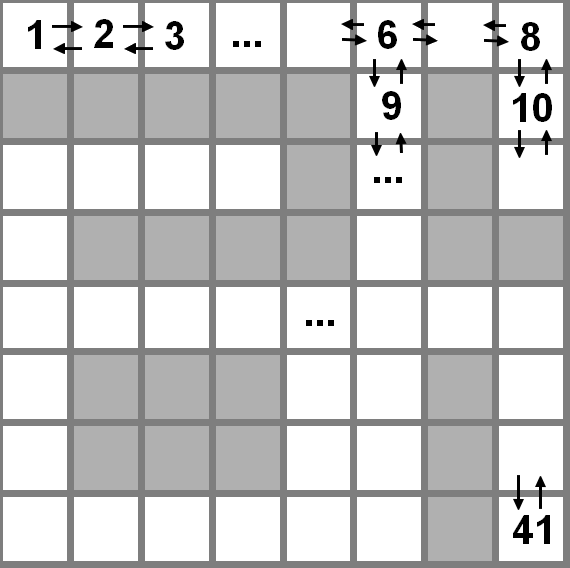
\includegraphics[width=5cm]{./images/lab.png}
			\caption{\textit{Modélisation du labyrinthe}}
		\end{wrapfigure}
		
		Dans l'exercice 3, on nous propose de résoudre des labyrinthes.\newline
		
		Intuitivement, le labyrinthe peut être modéliser par ce type de graphe. (voir figure)
		On crée un sommet pour chaque case 'non-mur' (cases vides, teleporteurs, porte, clef).
		Pour chaque sommet, on crée des arcs entre lui et ses voisins 'non-mur'.\newline
		
		Une fois le labyrinthe modélisé, il ne reste plus qu'à le résoudre à l'aide des algorithmes préalablement implementés.\newline
		
		\begin{algorithm}
			\caption{Résolution labyrinthe}
			\begin{algorithmic}
				\ENSURE Résout le labyrinthe.
				\REQUIRE $G = (X, A) ; A, S, C, P \in X ; t \in \Re$
						$E$ l'entrée, $E$ la sortie, $E$ la clef, $E$ la porte,
						$t$ le nombre d'action.
						$Dijkstra(X, E, S)$ une fonction de résolution de chemin le plus court allant de $E$ à $S$,
						renvoyant le nombre d'actions requit.\newline
				
				\textbf{Begin}
				
				\STATE Supprimer arcs de/vers la porte. (On considère la porte comme un mur)
				\IF {$Dijkstra(G, E, S) \leq t$}
					\STATE On a trouvé un chemin qui convient, sans passer par la porte. Fin.
				\ENDIF
				
				\STATE $t_1 \leftarrow Dijkstra(G, E, C)$
				\IF{$t_1 > t$}
					\STATE La clef est trop loin, pas de chemin. Fin.
				\ENDIF
				
				\STATE Créer arcs de/vers la porte. (On considère la porte comme une case vide)
				\STATE $t_2 \leftarrow t - t_1$
				\IF{$Dijkstra(G, C, S) < t_2$}
					\PRINT Un chemin de $E$ à $S$ passant par $C$ puis $D$ existe.
				\ELSE
					\PRINT Pas de chemin de $C$ à $S$ en moins de $t_2$ actions.
					\PRINT Donc, pas de chemin de $E$ à $S$ en moins de $t$ actions.
				\ENDIF
			\end{algorithmic}
		\end{algorithm}

		\newpage
		Voici les résultats de cet algorithme, appliqué au test exo3/06. (graphe de 1 000 000 de sommets,
		on cherche le plus court chemin entre les 2 sommets les plus distants)
	
		\begin{figure}[H]
			\begin{center}
				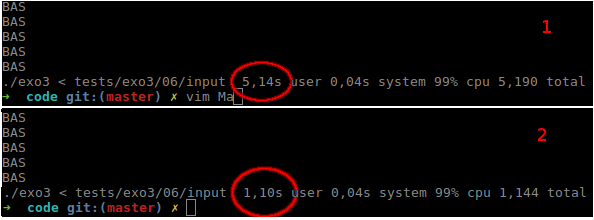
\includegraphics[width=11cm,height=\textheight,keepaspectratio]{./images/performances.png}
			\end{center}
			\caption{\textit{Temps d'execution des algorithmes}}
		\end{figure}
		
		Les algorithmes de résolution utilisé sont:
		
		\begin{itemize}[label=-]
			\setlength\itemsep{0.1em}
			\item 1 : Dijkstra sans file de priorité
			\item 2 : Dijkstra avec file de priorité
				\item 3 : A* avec file de priorité, et fonction heuristique ('rester sur la diagonal du labyrinthe')
		\end{itemize}
			
		\begin{figure}[H]
			\begin{center}
				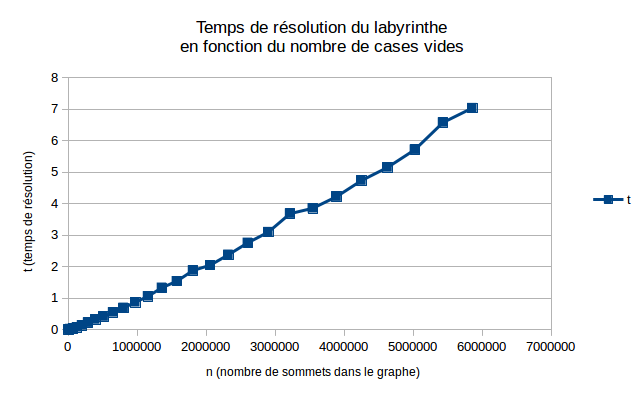
\includegraphics[width=12cm,height=\textheight,keepaspectratio]{./images/courbe_temps.png}
			\end{center}
			\caption{\textit{Temps de résolution de labyrinthe avec Dijkstra, allure en \(O(n * log(n))\)}}
		\end{figure}

	\newpage
	\section{A propos de l'implémentation}
		Ci joint, vous trouverez mon implémentation en language 'C'.
		\subsection{Structures de données}
		J'ai implémenté plusieurs structures de données, afin d'optimiser les algorithmes. Je les ai conçu de manière générique,
		afin de pouvoir m'en reservir plus tard dans d'autre projet. Si vous souhaitez plus de détail, je vous
		conseille vivement de regarder les fichiers '.c' et '.h', qui sont commentés.
		
		\subsection{Qualité logiciel}
			Mes programmes passent les tests fournis.\newline    
			De plus, j'ai debuggé l'integralité du code à l'aide de l'outil 'valgrind'.
			Il ne semble y avoir ni fuite mémoire, ni dépassement de tampon, ni accès à de la mémoire non initialisé.
			(tester sur le set de test fourni, avec des fichiers bien formattés).
			\begin{figure}[H]
				\begin{center}
					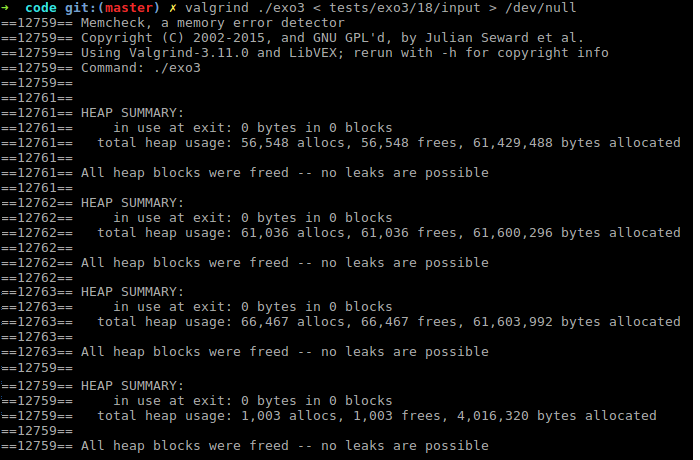
\includegraphics[width=12cm,height=\textheight,keepaspectratio]{./images/valgrind.png}
				\end{center}
				\caption{\textit{résultat de 'valgrind' sur 'tests/exo3/06')}}
			\end{figure}
			J'ai optimisé mon programme à l'aide de l'outil 'gprof'.
			D'où par exemple, l'implementation des tas binaires, ou du 'define' ARRAY\_ITERATE ('array.h')

	\newpage
	\section{Références}
		\begin{thebibliography}{}

			\bibitem{binary_heap}
				Wikipédia, Binary Heap, 15 Décembre 2017,\newline
				\href{https://en.wikipedia.org/wiki/Binary\_heap}
				      {\textit{https://en.wikipedia.org/wiki/Binary\_heap}}.

			\bibitem{priority_queues}
				Mary K. VERNON, Priority Queues, 3 Septembre 2016,\newline
				\href{http://pages.cs.wisc.edu/~vernon/cs367/notes/11.PRIORITY-Q.html}
					{\textit{http://pages.cs.wisc.edu/~vernon/cs367/notes/11.PRIORITY-Q.html}}.
		
			\bibitem{computerphile}
				Dr. Mike POUND, Sean RILEY, 24 Février 2017,\newline
				Maze Solving - Computerphile,\newline
				\href{https://www.youtube.com/watch?v=rop0W4QDOUI}{\textit{https://www.youtube.com/watch?v=rop0W4QDOUI}}.
			  
			\bibitem{heuristique}
				Wikipédia, Heuristique, 31 Octobre 2017,\newline
				\href{https://fr.wikipedia.org/wiki/Heuristique_(mathématiques)}
				      {\textit{https://fr.wikipedia.org/wiki/Heuristique\_(mathématiques)}}.
				      
			\bibitem{manhattan}
				Wikipédia, Distance de Manhattan, 31 Octobre 2017,\newline
				\href{https://fr.wikipedia.org/wiki/Distance_de_Manhattan}
				      {\textit{https://fr.wikipedia.org/wiki/Distance\_de\_Manhattan}}.

  \end{thebibliography}

\end{document}
